
\section{Videos}
\label{sec:org1f1f886}



\section{Posts}
\label{sec:org33c9a58}



\subsection{Set up the TikZ in Emacs Org}
\label{sec:org9a1a1dd}
\hspace{0pt}\\


An introduction to setup the TikZ environment in Emacs Org File. So that in Org file, you can generate either vector graph of \texttt{pdf}  format or raster graph of \texttt{png} format. Furthermore, you can export the vector graph when latex is called and otherwise raster graph.


\subsubsection{config the header args}
\label{sec:orgf59efeb}


You can embed TiKz (One of \(\LaTeX\) graphic package) code into a Org file. With
org-babel, you can generate ,insert and export the figure generated from Tikz
package. At first, you need set up the environment. \href{https://orgmode.org/worg/org-contrib/babel/languages/ob-doc-LaTeX.html}{This Post} serves as a good
introduction for beginners. Following it you may have a minimum working example
like below:

\begin{verbatim}
#+name: tutorial
#+header: :file "~/Dropbox/mstemc_hugo/static/img/tikz/tutorial.png"
#+header: :results raw :exports none :fit yes :border 0cm
#+header: :imagemagick t :iminoptions -density 400
#+header: :imoutoptions -geometry 400 -flatten
#+header: :headers '("\\usepackage{tikz} \\usetikzlibrary{positioning,
           shapes.symbols, calc}")
#+begin_src latex
  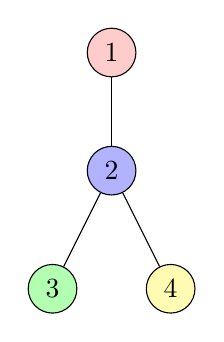
\begin{tikzpicture}
    \node [circle, draw, fill=red!20] at (0,0) {1}
    child { node [circle, draw, fill=blue!30] {2}
      child { node [circle, draw, fill=green!30] {3} }
      child { node [circle, draw, fill=yellow!30] {4} }};
  \end{tikzpicture}
#+end_src
#+RESULTS: tutorial
[[file:../../img/tikz/tutorial.png]]
\end{verbatim}

The example begins with several lines containing \texttt{\#+header} which is sort of
clutter. we can put them in a file and include it at the beginning of the Org
file.
\subsubsection{generate results with different formats}
\label{sec:orgebb7e4e}


By changing the extension of \texttt{:file} (which is \texttt{pdf} for
\texttt{"../../img/tikz/tutorial.pdf"} ), we can generate results with different formats.
Now, I need \texttt{pdf} and \texttt{png} . You can see the result by just press \texttt{C-c C-c} in the
body of the tikz code.
\subsubsection{export the results according to the backend}
\label{sec:org3858655}


You can set \texttt{:exports} to control how the results will be exported. Now I set it
as \texttt{none} which means the result will not be exported to latex or other format. I
want to set more options of the exports. So I use:

\begin{verbatim}
#+ATTR_HTML:  :width 800 :align center
#+ATTR_LATEX: :width 0.8\textwidth :align center
{{{if-latex(tutorial.pdf,tutorial.png)}}}
\end{verbatim}

\texttt{if-latex} is a Org MACRO whose definition is :
\begin{verbatim}
#+MACRO: if-latex (eval (if
(org-export-derived-backend-p org-export-current-backend 'latex)
 (concat "[[file:../../img/tikz/"  $1 "]]")
 (concat "[[file:../../img/tikz/"  $2 "]]") ))
\end{verbatim}

The \texttt{if-latex} MACRO let you export different formats by the backend. If the
backend is \texttt{latex} then, \texttt{pdf} format figure will be exported. Otherwise, \texttt{png} format
figure. Eventually, in the final \texttt{pdf} document, you figure can be zoomed in or
out without losing any resolution.

\subsubsection{the final workflow}
\label{sec:org2af511e}


The minimum working example at the start of this post is simplifed as below.

\begin{verbatim}
#+header: :file  "../../img/tikz/tutorial.pdf"
#+begin_src latex
  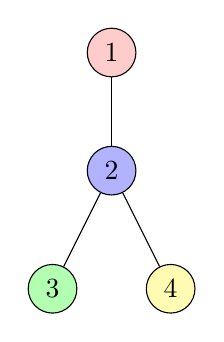
\begin{tikzpicture}
    \node [circle, draw, fill=red!20] at (0,0) {1}
    child { node [circle, draw, fill=blue!30] {2}
      child { node [circle, draw, fill=green!30] {3} }
      child { node [circle, draw, fill=yellow!30] {4} }};
  \end{tikzpicture}
#+end_src

#+RESULTS:
[[file:../../img/tikz/tutorial.png]]

The following is the generated figure.
#+ATTR_HTML:  :width 800 :align center
#+ATTR_LATEX: :width 0.8\textwidth :align center
{{{if-latex(tutorial.pdf,tutorial.png)}}}
\end{verbatim}

Many settings are grouped into a setup file which is included at the top of this
post:
\begin{verbatim}
#+SETUPFILE: ~/.spacemacs.d/org-templates/math-en.org
\end{verbatim}

Now, If you set the extension of the target file in the first line either \texttt{pdf} or
\texttt{png} , a corresponding \texttt{pdf} or \texttt{png} figure will be generated. If execute \texttt{M-x
org-toggle-inline-images}  , you can preview the result. If export the org-file
as latex file then the \texttt{pdf} file, the image of \texttt{pdf} format will be inserted. If
export to other format, \texttt{png} image will be used.



\subsection{Export Markdown and latex using Emacs Org}
\label{sec:orgf87a4ad}


\hspace{0pt}\\


set up the Emacs org and ox-hugo to export the org files in markdown and latex format.


\subsubsection{Introduction}
\label{sec:orgb9aacc7}


I use hugo before it support Emacs org file. Then I use an Emacs extension
called \href{https://github.com/kaushalmodi/ox-hugo}{ox-hugo} which is a carefully crafted Org exporter back-end for Hugo.
Ox-hugo meets all my requirement and definitely worth a try when you are an
advanced user of Emacs Org. By the way, if you are quite familiar with Emacs
Org, there is no need to take time to learn markdown. Emacs Org, I think, is
more elegant than markdown.

\subsubsection{set up ox-hugo}
\label{sec:org0a52bcd}


I use Spacemacs and integrate ox-hugo into my config is easy. You can add it
into your private layer or just add it in your \texttt{user-config} . Please refer to
\href{https://github.com/kaushalmodi/ox-hugo}{the repo.} and read the document for more information.

The first time you want to export an Org file or a subtree of an Org file, use
\texttt{M-x org-hugo-export-to-md} . There will be a hugo-related section in the
\texttt{org-dispatcher} whenever you use \texttt{C-c C-e} .
\subsubsection{use Org Macro replacement}
\label{sec:orgaa4e7a2}


Often, you want different actions when you export the Org file to
hugo-compatible markdown and latex file. For example, hugo or hugo theme supports
summary and shortcodes such as \texttt{alert note} and \texttt{alert warning} (see  \href{https://sourcethemes.com/academic/docs/writing-markdown-latex/}{Writing
content with Markdown, \LaTeX{}, and Shortcodes | Academic} )

When you export the snippet to markdown then hugo will display the content
according to the css. However, latex does not recognize the shortcodes. So latex
will display \texttt{\{ \{\% alert note \%\} \}} literally which is clutter. The Org Macro may
help. For more information please refer to \href{https://orgmode.org/manual/Macro-replacement.html}{The Org Manual: Macro replacement} and
\href{https://github.com/fniessen/org-macros}{fniessen/org-macros: Shared macros for Org mode} . I also define my own Org Macro
in \href{https://github.com/msteamc/.spacemacs.d/blob/master/org-templates/enpost.org}{my setup file for every .org file}. With Org Macro, I control some contents
and options exist only for certain backend.

Once you are familiar with Org Macro, It behaves beyond your imagination.
\subsubsection{use the setupfile for each Org file}
\label{sec:orgd15a7e2}


Often, you options for a org file grows more and more. If you think it kind of
clutter at the top of your Org files, you can group them in a setupfile then
include it at the top of your Org file.

For my setupfiles, please refer to \href{https://github.com/msteamc/.spacemacs.d/tree/master/org-templates}{my org-templates}. As you can see, I have
several setupfiles for different aims. To include one of them in my Org file, I
use:

\texttt{\#+SETUPFILE: <path+name of the setup files>}

By using \texttt{\#+SETUPFILE} ,I only have to option lines at the top of my org file.
So it looks clean.

Also, you can notice that in \href{https://github.com/msteamc/.spacemacs.d/blob/master/org-templates/enpost.org}{my setupfile named enpost.org} exists options for
different export targets.

\subsection{Drawing Graphs Using TikZ in Emacs Org}
\label{sec:org5bc49d6}



\subsubsection{Drawing a TikZ picture in Emacs Org Mode}
\label{sec:org8506b3a}


\lstset{language=[LaTeX]TeX,label=a-minimum-working-example,caption={a minimum working example},captionpos=b,firstnumber=1,numbers=left}
\begin{lstlisting}
\usetikzlibrary{intersections,arrows.meta}
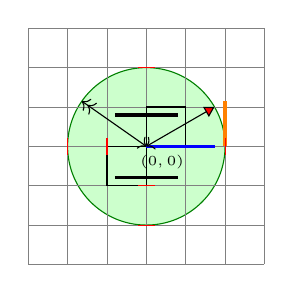
\begin{tikzpicture}[thin]
\draw (-1.5,0) -- (1.5,0);
\draw (0,-1.5) -- (0,1.5);
\filldraw[fill = green!20, draw = green!50!black] (0,0) circle[radius = 1cm];
\draw[help lines,very thin,step=.5cm,color=gray] (-1.5,-1.5) grid (1.5,1.5);
\draw (0,0) rectangle (.5,.5);
\draw (0,0) rectangle (-0.5,-0.5);
% relative coordinate
\draw[blue, very thick] (30:1) ++ (0,-0.5) --(0,0);
% name a path without drawing it
\path[name path = upward line] (1,0) -- (1,1);
\path[name path = sloped line] (0,0) -- (30:1.5cm);
% use intersection of two path
\draw[name intersections={of = upward line and sloped line, by=x}]
     [very thick, orange] (1,0) -- (x);
% use arrow
\draw[<->>] (0,0) -- (145:1);
\draw[<-{Triangle[fill=red]}] (0,0) -- (30:1);
% use scope
\begin{scope}[very thick]
\draw (-0.4,0.4) -- (0.4,0.4);
\draw (-0.4,-0.4) -- (0.4,-0.4);
\end{scope}
% use foreach
\foreach \x in {-1cm,-0.5cm,1cm}
    \draw[red] (\x,-3pt) -- (\x,3pt);
\foreach \y in {-1cm,-0.5cm,1cm}
    \draw[red](-3pt,\y) -- (3pt,\y);
% using node
\draw (0,0)+(0.2,-0.2) node {\tiny $(0,0)$ };
\end{tikzpicture}
\end{lstlisting}


\hspace{0pt}\\
The generated figure is shown as:
\begin{center}
\includegraphics[width=0.5\textwidth]{/Users/chaolongzhang/Dropbox/mstemc_hugo/static/img/tikz/example3.pdf}
\end{center}

\begin{enumerate}
\item In \hyperref[a-minimum-working-example]{the minimum working example} line 12 , a path is named  without drawing
it.
\item Line 16 gives an example of using library \texttt{intersections}. Note
that you need to add the library using \texttt{\textbackslash{}usetikzlibrary\{intersections\}}
otherwise an error occurs during \LaTeX compiling.
\item Line 18 and 19 gives an example of using arrow. To make it work,
\texttt{\textbackslash{}usetikzlibrary\{arrows.meta\}} is needed. The library \texttt{arrows.meta} provides tons
of types of arrows whick shock me when I see them the first time.
\item Line 21 to 24 gives an example of \texttt{scope} . In the environment, all
the lines are drawn in the \texttt{very thick} style.
\item Line 26 to 29 gives an examplt of \texttt{foreach} . \texttt{foreach} is handy
when you want to draw a list of objects. In \hyperref[a-minimum-working-example]{the minimum working example} , I
draw a list of short red sticks along with the x-axis and y-axis.
\item Line 31 is an example of \texttt{node}. The keyword \texttt{node} is typically followed by
some options between \texttt{[]} and then some text between \texttt{\{\}}. Every node has flexible
anchor options to decide where the text should be placed.
\end{enumerate}
\subsubsection{Another Example}
\label{sec:org85bdcaf}


The code is shown as:
\lstset{language=[LaTeX]TeX,label=another-minimum-working-example,caption={another minimum working example},captionpos=b,firstnumber=1,numbers=left}
\begin{lstlisting}
\usetikzlibrary{intersections,arrows.meta}
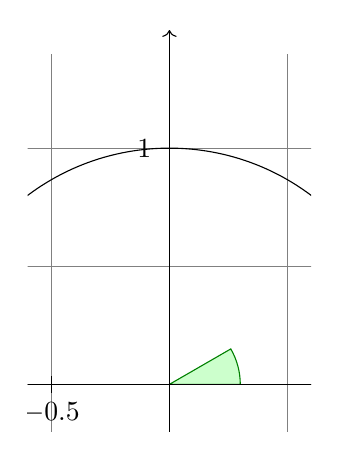
\begin{tikzpicture}[scale=3]
  \clip (-0.6,-0.2) rectangle (0.6,1.51);
  \draw[step = .5cm, help lines] (-1.4,-1.4) grid (1.4,1.4);
  \filldraw[fill=green!20,draw = green!50!black] (0,0) -- (3mm,0mm)
  arc [start angle = 0, end angle = 30,radius = 3mm] -- cycle;
  \draw[->] (-1.5,0) -- (1.5,0);
  \draw[->] (0,-1.5) -- (0,1.5);
  \draw (0,0) circle [radius=1cm];
  \foreach \x in {-1,-0.5,1}
  \draw(\x cm, 1pt) -- (\x cm, -1 pt) node [anchor = north] {$\x$};
  \foreach \y in {-1,-0.5,1}
  \draw(1pt,\y cm) -- (-1pt, \y cm) node[anchor = east] {$\y$};
\end{tikzpicture}
\end{lstlisting}

The generated figure is shown as:
\begin{center}
\includegraphics[width=0.5\textwidth]{/Users/chaolongzhang/Dropbox/mstemc_hugo/static/img/tikz/example4.pdf}
\end{center}


\subsubsection{Some Basic Rules in TikZ}
\label{sec:orge995912}


\begin{enumerate}
\item The options appear in \texttt{[]}. No matter it is an object or an operation, the
contents in the following  \texttt{[]} serve as options.

Options \texttt{[]} can be at the very beginning of the environment \texttt{tikzpicture}
following the operation, following the object.

\item \texttt{\textbackslash{}filldraw} is a good command. It draws a closed loop and fill it with color or
pattern. The colors for filling and drawing can be different.

\item Coordinates can be specified in x-y format, polar format.
\begin{itemize}
\item The easiest way is \texttt{(x,y)} which means \texttt{x} cm in the x-axis and \texttt{y} cm in the
y-axis;
\item \texttt{(a:x)} is the polar format which means \texttt{x} cm in direction \texttt{a} degree.
\end{itemize}
\item \texttt{(<p> |- <q>)} is another way to specify coordinates for example \texttt{(30:1 |- 0,0)}
which means the interaction of a vertical line through \texttt{(30:1)} and a
horizontal line through \texttt{(0,0)} .
\item Relative coordinates are possible with \texttt{+} and \texttt{++} in front of \texttt{(x,y)} and \texttt{(a:x)} .
\texttt{+} is relative to the closest coordinate whereas \texttt{++} is relative to the very
first coordinate of current path.
\end{enumerate}

\subsubsection{Some tips for in TikZ}
\label{sec:org742f086}


\begin{enumerate}
\item To use \texttt{intersections} to specify a coordinate, you need to include the
library, i.e. \texttt{\textbackslash{}usetikzlibrary\{intersections\}} is a must.
\end{enumerate}

\lstset{language=C,label= ,caption= ,captionpos=b,firstnumber=1,numbers=left}
\begin{lstlisting}
int main()
{
  int i=0;
  printf();
}
\end{lstlisting}

\bibliography{../../research_library/zcl}
\bibliographystyle{unsrt}

\subsection{Walk Through the Petri-Net In TiKZ Tutorial}
\label{sec:orgfaa8657}


\bigin{titlepage}
 \begingroup
\begin{center}
 \vspace{\baselineskip}
 \textbf{\Huge Walk Through the Petri-Net In TiKZ Tutorial} \par
 \vspace{2\baselineskip}  \newline
 \textbf{\large Eason Zhang with www.makesteamclear.com \par}
 \vspace{\baselineskip}          \newline
  \today \par
 \vspace{\baselineskip}
  \vfill
 \setlength{\unitlength}{3pt}
 \includegraphics[width=0.5\textwidth]{/Users/chaolongzhang/Dropbox/mstemc_hugo/static/img/tikz/example3.pdf}
 \vfill \vspace{\baselineskip}
 \href{WWW.MAKESTEAMCLEAR.COM}{\Large WWW.MAKESTEAMCLEAR.COM} \par\newline
  www.makesteamclear.com is a free project, supported by Eason Zhang, to make videos about STEAM in a more approachable and different way. If you found the contents in this post or the site or the youtube channel helpful, please consider \href{www.makesteamclear.com}{support me}, thanks \par
 \end{center}
\endgroup
\end{titlepage}
\newpage

Chapter 3 of the TikZ tutorial gives an example of Petri net. In this post, let
me work through the code line by line. During this example, more tikz libraries
are used, such as \texttt{arrows} , \texttt{decorations.pathmorphing} , \texttt{backgrounds} ,
\texttt{positioning} , \texttt{fit}, \texttt{petri} . These libraries should be added before the
\texttt{tikzpicture} environment.

\begin{center}
\includegraphics[width=0.8\textwidth]{/Users/chaolongzhang/Dropbox/mstemc_hugo/static/img/tikz/petrinet.pdf}
\end{center}



\section{Projects}
\label{sec:orgaf97de2}


\subsection{my workflow of creating a video}
\label{sec:org45aac98}
\hspace{0pt}\\


This collection of Videos and Posts describes my workflow of creating a video. Usage of some tools and methods are covered.


During the creation of one video, several tools are tuned to fit my workflow. In
this project several videos and posts will be created to make my workflow clear.

Two targets of this project:
\begin{enumerate}
\item remind me of the configuration of several tools;
\item show somebody else who may be interested in how I work.
\end{enumerate}

I am not ready to detail each tool. If you are interested in any one of them,
please refer to tutorials written by experts or given by the official document.

\subsubsection{Emacs}
\label{sec:orgcb16fe3}


Emacs lies in the center of my workflow. It behaves like a super-IDE which
assists me finish almost all the steps. Using Emacs, I program and debug, GTD,
write the blogs, export and publish them. Many of the Emacs extensions are
awesome. In particular, Emacs Org is the killer app.

How to config Emacs? After more Than ten years of using Emacs, I choose
spacemacs. Most beginners can start their work using spacemacs with only a
little modifications.

\begin{enumerate}
\item program and debug
\label{sec:orgbe5b8cf}


I program in python, C/C++, Matlab and some other languages. Emacs acts as a
super-IDE for me.


\item Org mode - journalize your work
\label{sec:org5077380}


Org mode definitely need a standalone subsection.

\item Org mode - get things done
\label{sec:org0286871}



\item Org mode - write a diary
\label{sec:org2d64073}

\item Org mode - export your Org file
\label{sec:orgbd13d0c}


\item program and debug
\label{sec:org53b4991}


\item writing latex
\label{sec:orgce5ad4a}
\item org-journal
\label{sec:orgb58b60d}


I write many notes during a post or a project. Most of my journal is maintained
by \href{https://github.com/bastibe/org-journal}{org-journal: A simple org-mode based journaling mode} . And I set the
\texttt{org-journal-file-type} to \texttt{weekly} So that I have around 52 journal file each
year.

The journals can be searched conveniently. Also they can be integrated into Org
agenda.


\item ox-hugo
\label{sec:org7fc8972}


\href{https://github.com/kaushalmodi/ox-hugo}{kaushalmodi/ox-hugo: A carefully crafted Org exporter back-end for Hugo}

Because hugo supports markdown at first (it also supports org file later), I use
Emacs Org from the very beginning. I am quite familiar with org-mode, so have no
motivation to dig into markdown. Fortunately, ox-hugo meets all my requirement
and definitely worth a try when you want to stay in Org.

Actually, Emacs have extensions to support markdown quite well. However, using
Org, I can integrate the org file into my agenda.


\item preview tikz picture in Org
\label{sec:org697542b}


\href{http://www.texample.net/tikz/}{TikZ and PGF} are \TeX{} packages for creating graphics programmatically. TikZ is
build on top of PGF and allows you to create sophisticated graphics in a rather
intuitive and easy manner.

You can integrated TikZ code into the Org mode as a source block. I have a
not-so-detailed post on how to set up the tikz environment in Org.
\end{enumerate}


\subsubsection{Hugo}
\label{sec:org7cb7cf9}


As the fastest framework for building websites, Hugo shocks me by its speed and
flexibility. It is enough to prettify your site using the more than 300+
beautiful themes, from which I am in the mode for Academic theme.

Hugo supports Org file but not so good. Ox-hugo, another extension of Emacs, has
my attention. Serving as a bridge between Emacs and Hugo, ox-hugo helps me
staying in Emacs Org. There is no need for me to write markdown file if Org is
available.

I use ox-hugo as a bridge between Emacs and Hugo. So I do not have to care much
about how to leverage Hugo. Ox-hugo helps me do most of the work.
\subsubsection{Hugo Academic Theme}
\label{sec:org8323bc3}


\href{https://github.com/gcushen/hugo-academic}{Hugo Academic Theme} is a beautiful and flexible theme developed for Hugo. This
site is built based on this theme.

If you want attach a pdf version of your post, two steps are needed:
\begin{enumerate}
\item add a line:
\begin{verbatim}
url_pdf = "#"
\end{verbatim}
in the front matter of your markdown file.
\item add a PDF file with the same name as your post’s own folder to your post’s
folder.
\end{enumerate}

A PDF link will be automatically generated just like the \texttt{pdf} link appears in
the top of each post in my site. Because I use Emacs Org with ox-hugo, I add one
line in the property:

\begin{verbatim}
:EXPORT_HUGO_CUSTOM_FRONT_MATTER+: :url_pdf "#"
\end{verbatim}

Hugo academic theme provide some front matters that hugo does not support by
default. Fortunately, \href{https://github.com/kaushalmodi/ox-hugo}{ox-hugo} handles this effectively. For more information.
you can read:
\begin{enumerate}
\item \href{https://ox-hugo.scripter.co/doc/org-meta-data-to-hugo-front-matter/}{Org meta-data to Hugo front-matter}
\item \href{https://ox-hugo.scripter.co/doc/custom-front-matter/}{Custom Front-matter Parameters}
\end{enumerate}


\subsubsection{manim}
\label{sec:org00574e3}



\subsubsection{blender}
\label{sec:orgbef2b43}

\section{Courses}
\label{sec:orgeb1cbcd}
